\chapter{背景及相关研究}\label{chap:background}
本章首先概述GPU体系结构的相关知识和研究人员在不同GPU架构上实现的矩阵乘算法,引出AMD GPU矩阵乘相关的背景知识。然后介绍目前国内外对GPU矩阵乘的调优工作。最后一小节介绍本文工作所采用的AMD GPU体系结构的相关知识,以帮助理解本文中使用的矩阵乘调优方法。

\section{GPU架构概述}

GPU(Graphics Processing Units)设计之初是为了做图形渲染。在图像渲染中,大部分工作是在进行顶点和像素的处理,由于顶点和像素处理具有天然的并行性,所以GPU的发展方向就是大量“轻型”线程,可以快速进行任务切换。由于具有大量并行“轻量”线程的特点,以及复杂的硬件动态调度,是的GPU具有很好的延迟容忍特性。

从线程的概念上,GPU的线程由应用程序,驱动,运行时库和硬件调度器进行控制。GPU的线程更为底层,接近硬件。CPU端的线程更为上层,由操作系统控制线程的创建,调度和回收等工作。

从应用场景上,GPU可以分为移动端,桌面端和服务器级GPU。移动端GPU的特点是要做到功耗,同时也要具有较高计算性能。桌面端和服务器级GPU则追求更高计算性能,对功耗则没有非常苛刻的要求。为了实现高访存带宽,GPU的大量引脚被用来连接内存,并且使用GDDR5高带宽访存协议。

在计算单元的设计上,AMD和NVIDIA GPU的计算单元都采用了SIMD(Single Instruction Multiple Data)(或者SIMT Single Instruction Mulitiple Thread)架构。在术语上,AMD称其为SIMD,NVIDIA称其为SIMT或SPMD(Single Program Multiple Data)。AMD GPU由很多CU(Compute Units)组成,NVIDIA GPU由很多SM(Streaming Multi-processors)或SMX组成。对于AMD Redeon Vega10架构,每个CU有4个SIMD部件,每个SIMD的宽度为16。通过向量流水线的方式用4个时钟周期来执行宽度为64的向量操作。对于NVIDIA GTX780,其设计为Kepler架构,每个SMX有12个SIMD,每个SIMD的宽度为16。通过2个时钟周期来执行宽度为32的向量操作。

对于AMD GPU GCN架构,每个CU包含一个标量部件和4个SIMD部件,每个SIMD最多可以有10个向量线程(AMD称为wavefronts)in flight,向量线程的宽度为64。一个SIMD在每个指令发射周期选择一个向量线程来执行。所以,一个CU最多可以运行40个向量线程。NVIDIA GPU在设计上也与之类似。但实际可运行的向量线程数受很多因素限制,这里包括寄存器数量,局部共享内存的大小等。

对于AMD GPU和NVIDIA GPU体系结构,采用了SIMD的编程模型,每个线程是SIMD中的一项。NVIDIA称之为“SIMT(Single Instruction, Multiple Thread)”或者“SPMD(Single Program, Multiple Data)”。对于AMD GPU,一个wavefront有一个程序计数器,指令的分支由专门的寄存器做掩码来标记,控制每个线程的行为。

通过上面的比较,可以看出,AMD GPU和NVIDIA GPU都采用了SIMD结构,不同的是AMD GPU所计算的向量的宽度为64,NVIDIA GPU所计算的向量宽度为32。由此可以窥见SIMD结构代表着现代GPU的主流设计方向。




\section{GPU线程执行模型}
本文旨在基于AMD GPU平台,对矩阵乘算法进行实现和优化。为了实现更高效的矩阵乘,编程人员必须深入分析GPU体系结构的组织方式和GPU程序的编程和执行模型。

GPU程序的逻辑调度和执行单元是block,在术语上,NVIDIA称为thread block或block,AMD称为work-group。一个block中的所有线程共享一个shared memory。在硬件上,一个block执行时位于某一个SMX(CU)中。Block的执行不能跨SMX(CU)。一个block包含一到多个warp(wavefront)。一到多个block组成一个grid(NDRange)。如图\ref{fig:thread_model}展示了AMD GPU线程的组织方式。一个warp有32个线程,wavefront有64个线程,OpenCL中称为work-item。

\begin{figure}[htbp]
	\centering
	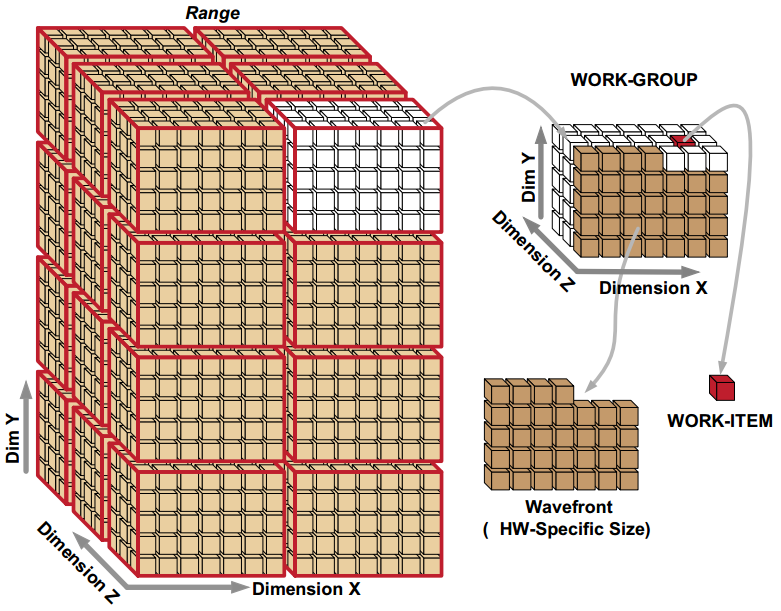
\includegraphics[width=0.50\textwidth]{thread_model}
	\bicaption{work-item,wavefront和NDRange之间的关系}{The relationship between work-item, wavefront and NDRange}
	\label{fig:thread_model}
\end{figure}

在线程执行模式上,NVIDIA GPU以warp为单元调度和执行,一个warp有32个线程。一个warp中的线程协作执行。AMD GPU以wavefront为单元调度,一个wavefront有64个线程(如图\ref{fig:warp_model})。在warp(wavefront)执行过程中,遇到分支时,在时间上来看,是“串行”执行的(如图\ref{fig:if_else},\ref{fig:warp_if_else})。

\begin{figure}[htbp]
	\centering
	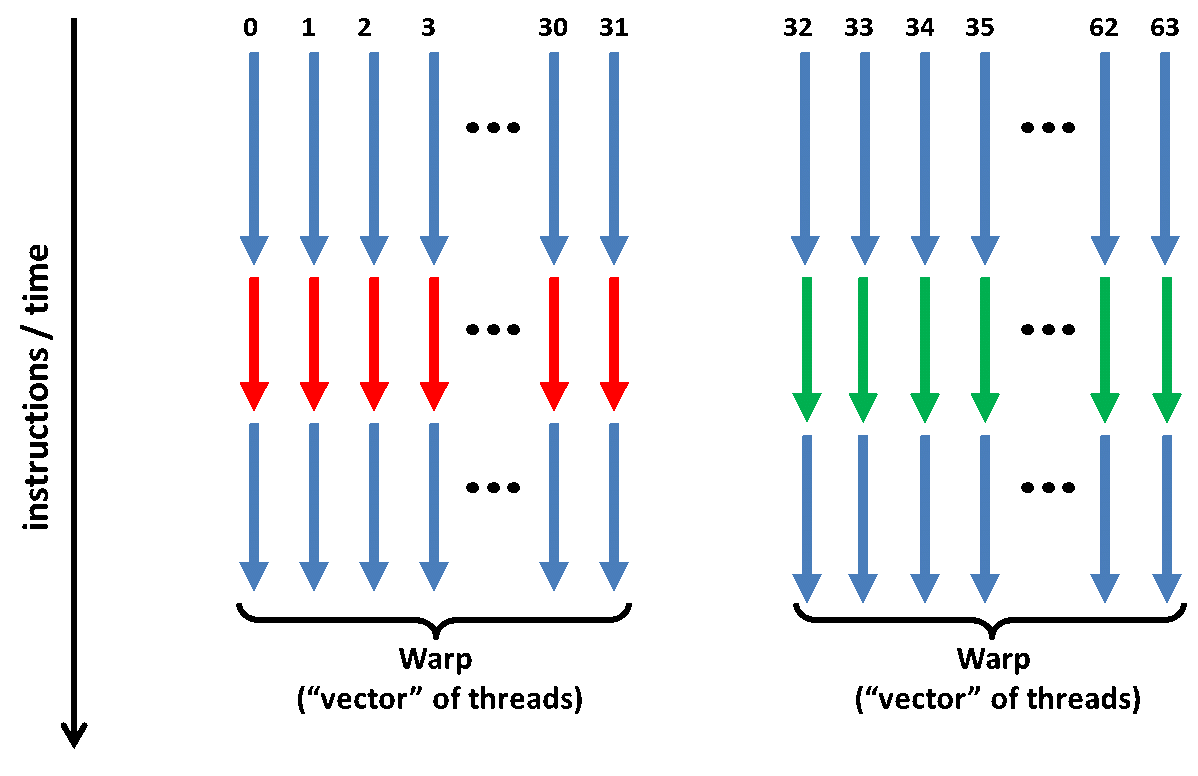
\includegraphics[width=0.50\textwidth]{warp_model}
	\bicaption{NVIDIA warp执行模式}{NVIDIA warp execution model}
	\label{fig:warp_model}
\end{figure}


\begin{figure}[htbp]
	\centering
	%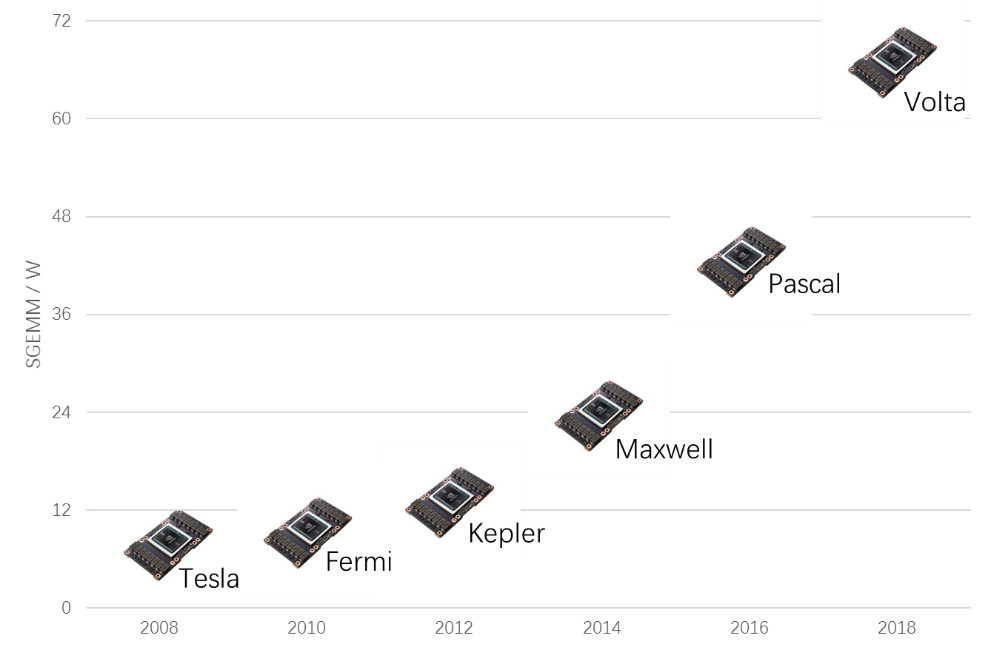
\includegraphics[width=0.40\textwidth]{nvidia_roadmap}
	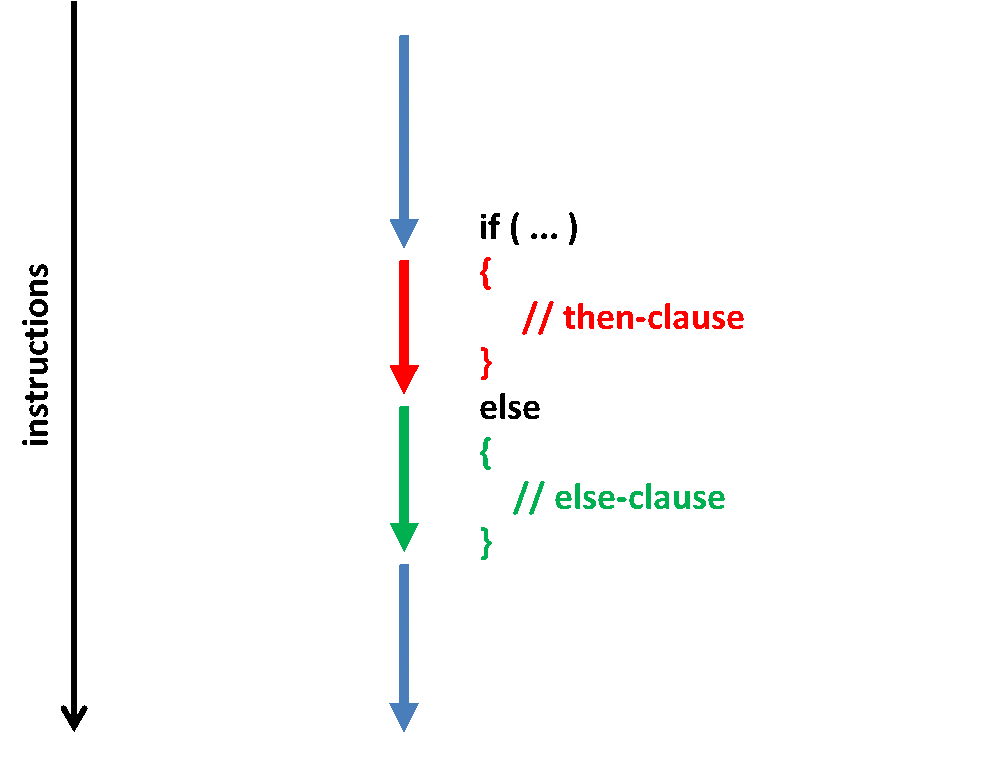
\includegraphics[width=0.50\textwidth]{if_else}
	\bicaption{if-else分支控制流}{If-else branch control flow}
	\label{fig:if_else}
\end{figure}

\begin{figure}[htbp]
	\centering
	%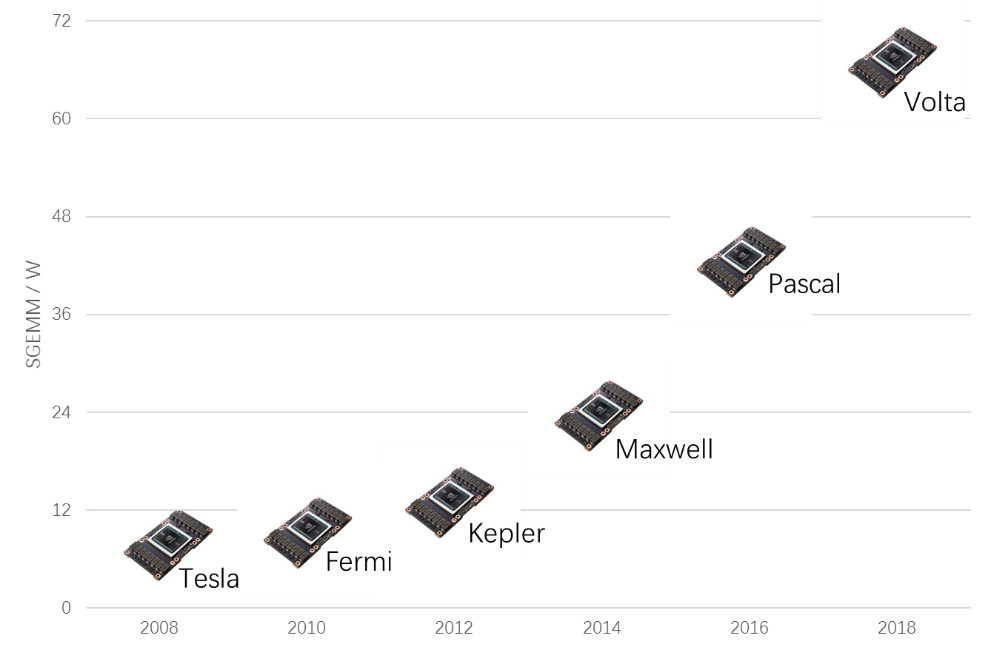
\includegraphics[width=0.40\textwidth]{nvidia_roadmap}
	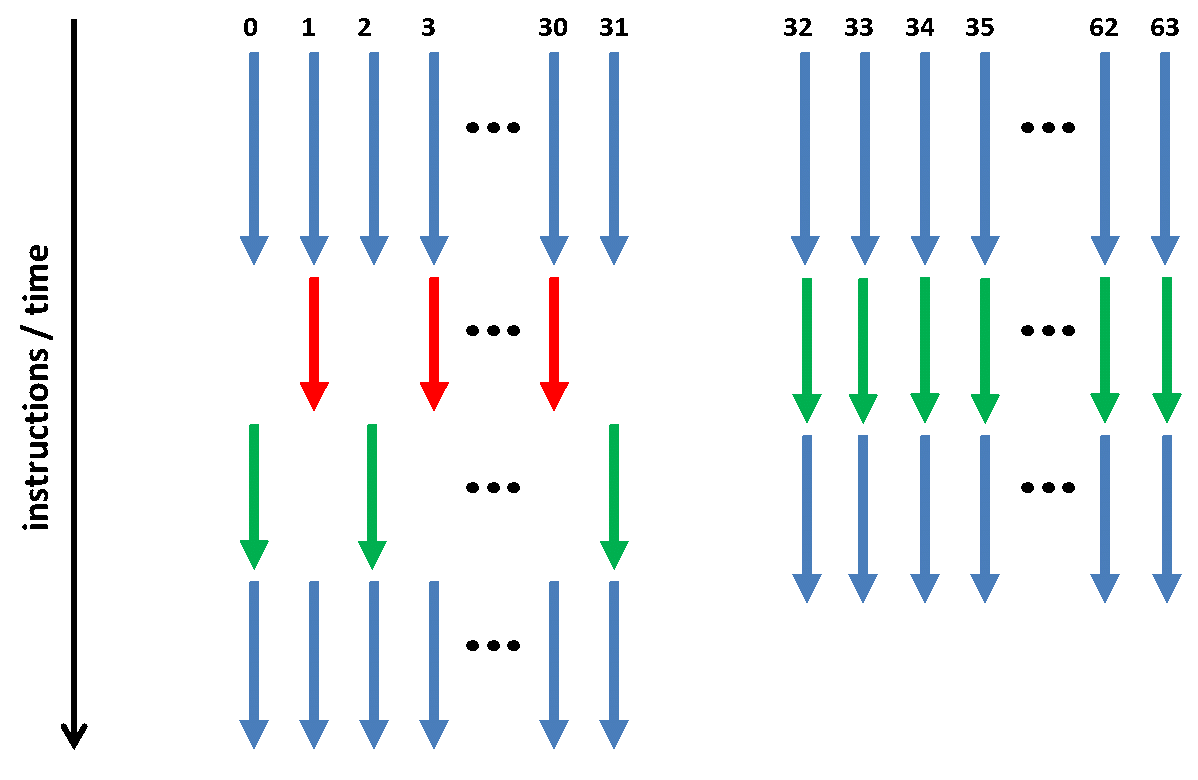
\includegraphics[width=0.50\textwidth]{warp_if_else}
	\bicaption{warp(wavefront)执行if-else分支流图}{Warp(wavefront) executes if-else branch flow graph}
	\label{fig:warp_if_else}
\end{figure}

由此,可以看出在设计GPU程序时,尽量减少指令分支。因为分支将导致程序“串行”执行,极大降低了执行速度。在接下来的章节里,将讨论如何设计GPU程序,以使线程的执行步调尽可能一致。从而提高执行速度。

\section{现有矩阵乘调优工作}
在本小节中,首先给出矩阵乘的标准数学表达,然后介绍现有矩阵乘在多核处理器上的研究工作。

\subsection{矩阵乘数学定义}
矩阵乘(GEMM General Matrix Multiply)数学表达为

\begin{equation}
	C:= \alpha op(A)*op(B) + \beta C
\end{equation}

其中A,B,C为矩阵,$\alpha$,$\beta$ 为标量。op 表示矩阵是否转置。即 op(X) = X 或 op(X) = $\mathbf{X}^\mathrm{T}$

\subsection{矩阵乘在多核处理器上的研究介绍}
目前国内外对矩阵乘的调优工作主要集中在NVIDIA GPU和各种主流CPU。NVIDIA在2010年设计出了第一款Fermi架构GPU。Fermi架构也影响着此后NVIDIA GPU架构的演变。Volkov\citepns{volkov2008benchmarking}通过benchmark的方法做了8系列,9系列和200系列NVIDIA GPU矩阵乘调优工作。

Junjie Lai\citepns{lai2013performance}在Fermi和Kepler架构上通过SGEMM(Single-precision General Matrix Multiply)算法性能分析和汇编级的微基准程序测试,提出了一套分析GPUs应用程序性能上界的方法。Junjie Lai通过分析发现,Fermi(Kepler)指令集自身的特点和调度器有限的发射通量是限制SGEMM通向理论峰值的两个主要因素。Lai评估了SGEMM的性能上界在GTX580 Fermi GPU为理论峰值的82.5\%,在GTX680 Kepler GPU为理论峰值的57.6\%。

Scott实现了第一个NVIDIA Maxwell架构开源汇编器MaxAs\citepns{grayassembler}。基于该汇编器,手写了非常高效的矩阵乘和卷积kernel。其实现的SGEMM在Maxwell架构上达到理论吞吐量的98\%,比NVIDIA官方库cuBLAS\citepns{nvidia2008cublas}汇编矩阵乘要快4.8\%。并写了一个微基准测试框架,为指令调度做铺垫。在开始这项工作之前,Scott仔细研究了cuBLAS在Kepler和Maxwell架构上的矩阵乘实现。Maxas SGEMM是Junjie Lai工作的一个扩展,针对Maxwell架构做了汇编级的调优。相比于Lai的工作,Scott破解的了Maxwell架构汇编控制码的含义,为实现更细粒度指令调度提供了可能。Scott在64线程的矩阵乘实现中,计算得出的矩阵乘性能上界为98.5\%(表\ref{tab:maxwellFFMA})。
\begin{table}[htbp]
	\bicaption{矩阵乘主循环指令构成}{GEMM main loop instructions}
	\label{tab:maxwellFFMA}
	\begin{center}
		\begin{tabular}{ | l | p{3cm} |}
			\hline
			Operation & Count \\ \hline
			FFMA & 512  \\ \hline
			LDS.128 & 32 dual issue \\ \hline
			STS.128 & 4 dual issue \\ \hline
			TLD.128 & 4 dual issue \\ \hline
			IADD & 4 \\ \hline
			XOR & 3 \\ \hline
			SETP & 1 \\ \hline
			BAR & 1 dual issue \\ \hline
			BRA & 1 daul issue \\
			\hline
		\end{tabular}
	\end{center}	
\end{table}

FFMA通量为512/(512+4+3+1)=512/520 = 98.5\%。其他指令是双发射的,不计入计算中。其中,指令的双发射由控制码进行控制。

Zhang\citepns{zhang2017understanding}实现了Kepler架构第一个开源汇编器KeplerAs\citepns{xiuxiaassembler},填补了Kepler GPU无可用汇编器的现状。Zhang在Scott和Lai工作的基础上,破解了Kepler K20 GPU架构的控制码,探测出Kepler GPU寄存器bank分布。利用Kepler架构独有的FFMA双发射,在NVIDIA kepler K20m上实现了更快的SGEMM,性能为3.1Tflop/s,达到88\%的计算效率,高出cuBLAS7.0 15\%。优化的卷积高出cuDNN4.0 39\%$\sim$62\%。

德州大学奥斯汀分校的Goto等人在2005年编写了基本线性代数库GotoBLAS。在BLAS Level-3中针对GEMM(General Matrix Multiply)做了优化。GotoBLAS作者在2010年去了微软工作,之后GotoBLAS停止了更新和维护。在2011年中科院软件所张先轶等人基于GotoBLAS发起了OpenBLAS\citepns{xianyi2012openblas}项目,OpenBLAS在各种主流CPU上都获得了比较高的性能。以OpenBLAS库为核心技术的彭峰科技取得了商业上的成功。但OpenBLAS主要针对CPU端做了十分细致的优化,而在GPU上做的优化工作则比较少。


\section{本章小结}
本章首先概述GPU体系结构的相关知识和研究人员在不同GPU架构上实现的矩阵乘算法,引出AMD GPU矩阵乘相关的背景知识。然后介绍矩阵乘的数学定义,目前国内外GPU矩阵乘的调优工作。最后一小节介绍本文工作所采用的AMD GPU体系结构的相关知识,以帮助理解本文中使用的矩阵乘调优方法。




